% ============================================================
%  NCRTHT 2026 submission (4-page IEEE double-column limit).
%  Condensed from paper/main.tex. Every number is taken from results/rigor_report*.json;
%  verify with: uv run python -m scripts.check_paper_numbers --tex paper/main_ncrtht2026.tex
% ============================================================
\documentclass[conference]{IEEEtran}

\usepackage{cite}
\usepackage{amsmath,amssymb,amsfonts}
\usepackage{graphicx}
\usepackage{textcomp}
\usepackage{xcolor}
\usepackage{booktabs}
\usepackage{array}
\usepackage{url}
\usepackage{newtxtext,newtxmath}  % Times, as IEEEtran prescribes (XeTeX cannot load IEEEtran's ptm fonts)
\usepackage[hidelinks]{hyperref}


\begin{document}

\title{Do Governance Checks Improve Clinical Question-Answering Accuracy? A Paired Evaluation of Multi-Agent Language Models}

\author{\IEEEauthorblockN{Areddy Divya Reddy}
\IEEEauthorblockA{\textit{Dept. of AI and Machine Learning} \\
\textit{Malla Reddy University}\\
Hyderabad, India \\
areddy.divya@mallareddyuniversity.ac.in}
\and
\IEEEauthorblockN{Namburi Rishika}
\IEEEauthorblockA{\textit{Dept. of AI and Machine Learning} \\
\textit{Malla Reddy University}\\
Hyderabad, India \\
rishikanamburi@gmail.com}
\and
\IEEEauthorblockN{Nooka Nikshith}
\IEEEauthorblockA{\textit{Dept. of AI and Machine Learning} \\
\textit{Malla Reddy University}\\
Hyderabad, India \\
nikshithnooka@gmail.com}
\and
\IEEEauthorblockN{Peddireddy Venkata Sujitha Sree}
\IEEEauthorblockA{\textit{Dept. of AI and Machine Learning} \\
\textit{Malla Reddy University}\\
Hyderabad, India \\
sujithashree3105@gmail.com}
}

\maketitle

\begin{abstract}
A common safeguard for language-model decision support is to surround the model with further agents that verify,
check safety and review its answer. We test whether such governance improves the accuracy of the final answer. Using GovBench-Clinical, an open
harness, we ran 300 MedQA-USMLE questions with their original answer key through a baseline (G0), all checks attached
as warnings (G4 open loop), and four closed-loop configurations in which a blocking finding sends the diagnosis back
for one revision. Every configuration started from the same first diagnosis, so differences come from governance
alone. Accuracy was 43.0 percent without checks and with checks as warnings, but fell to 37.3 percent when all
checks could trigger revision: revisions fixed 21 answers and broke 39. This exploratory drop is significant only
before correction (McNemar p = 0.040) and not after Holm correction across 30 paired tests (p = 0.55). No single
check improved accuracy significantly. The checks did not separate right from wrong answers, with an area under the
receiver operating characteristic curve of 0.497 to 0.57, and the safety validator raised an alert on every run of
each configuration that included it. Governance raised mean tokens per question from 2200.9 to 11362.7. An earlier
unpaired pass, which regenerated the first diagnosis, showed apparent gains that disappeared under pairing.
Governance signals need validation on paired data before revision is built on them.
\end{abstract}

\begin{IEEEkeywords}
Clinical decision support, large language models, multi-agent systems, AI governance, healthcare applications,
evaluation methodology.
\end{IEEEkeywords}

% ============================================================
\section{Introduction}
% ============================================================
Large language models (LLMs) now pass licensing-style medical examinations~\cite{singhal2023large,nori2023capabilities} and
are proposed as clinical decision support~\cite{rajpurkar2022ai}, including as a possible second opinion where
specialists are few. Because fluent models still state wrong findings or recommend unsafe
management~\cite{hager2024evaluation,pal2023medhalt}, many systems add further agents that critique or check its
output~\cite{hong2023metagpt,wu2023autogen,du2023improving}. These layers cost tokens and time, which could matter
where compute is limited, so their benefit has to be measured, not assumed~\cite{bedi2025optimization}. We measure
answer accuracy on exam questions, not deployment feasibility, accessibility or patient outcomes.

Our contributions are: (1) a \emph{paired} closed-loop experiment on 300 MedQA questions, in which revising on
governance feedback did not raise accuracy, whereas an unpaired pass showed apparent gains; (2) evidence that the
governance signals barely separate right from wrong answers, which explains why acting on them does not help; and
(3) GovBench-Clinical, an open harness with per-agent token, latency and cost reporting, and an audit of how lenient
string scoring inflated our own earlier results.

% ============================================================
\section{Related Work}
% ============================================================
MedQA~\cite{jin2021medqa} and PubMedQA~\cite{jin2019pubmedqa} score a single model's answer but not the checks placed
around it. Multi-agent frameworks~\cite{hong2023metagpt,wu2023autogen,chen2023agentverse} and multi-agent
debate~\cite{du2023improving} decompose a task across agents; MedAgents~\cite{tang2024medagents} and
MDAgents~\cite{kim2024mdagents} apply this to medicine, and MedAgentBoard~\cite{zhu2025medagentboard} finds that
multi-agent designs do not consistently beat simpler methods. Bedi et al.~\cite{bedi2025optimization} show that
improving clinical agents one component at a time does not guarantee a better system. Guardrail
toolkits~\cite{rebedea2023nemo} and LLM-as-a-judge evaluation~\cite{zheng2023judging} are widely used; we evaluate
governance by whether it changes, and improves, the final answer.

% ============================================================
\section{System}
% ============================================================
Fig.~\ref{fig:arch} shows the pipeline. A research agent extracts structured findings from the case text (it does not
retrieve literature) and a diagnosis agent chooses an answer and a ranked differential. Up to three checks then run in
parallel on this first answer: a grounding verifier flags claims the case does not support, a safety validator lists
safety concerns with a severity, and a consistency checker compares the extracted findings with the diagnosis. A
simulated attending reviewer, a language model and not a clinician, then reads the case, the diagnosis and the safety
findings and approves, rejects or requests revision. Deterministic contraindication rules add flags to every final
answer without changing it. All agents share one model.

\begin{figure*}[t]
\centering
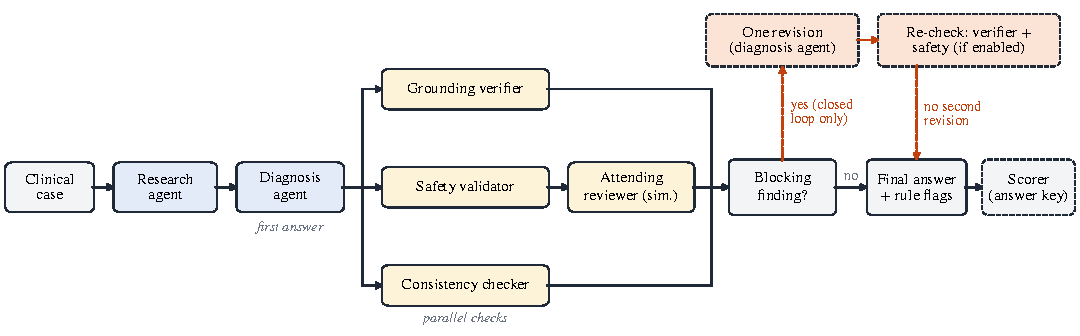
\includegraphics[width=\textwidth]{figures/architecture.pdf}
\caption{Workflow of G4 (all checks); G1--G3 enable one check each and G0 none. In open loop, findings are attached
to the output and the answer is never changed. In closed loop, any blocking finding triggers exactly one revision by
the diagnosis agent; the verifier and safety validator, when enabled, then re-check the revised answer, but their
findings cannot trigger a second revision. Only the scorer reads the answer key.}
\label{fig:arch}
\end{figure*}

The levels are G0 (no checks), G1 (verifier), G2 (attending reviewer), G3 (safety validator) and G4 (all of these plus
the consistency checker). G1--G3 are alternative single mechanisms, not a strict hierarchy. In closed loop, an
ungrounded claim, a HIGH or CRITICAL safety concern, a severe contradiction, or a request to revise or reject triggers
exactly one revision; an unparseable revision would keep the original answer and be recorded as a failure (none
occurred).

% ============================================================
\section{Experimental Setup}
% ============================================================
\textbf{Data.} We sampled 300 questions (seed 42) from the 1,273-question four-option test set of MedQA-USMLE
(United States Medical Licensing Examination)~\cite{jin2021medqa}, keeping the original options and answer key. Only the scorer reads the key; a test confirms
that no agent prompt contains it.

\textbf{Model.} Every agent used Llama-3.2-11B-Vision-Instruct on the NVIDIA NIM API,
at temperature 0.1 for extraction and checks and 0.2 for diagnosis, revision and review, with at % numcheck:ignore
most 1{,}500 output tokens per call. We ran G0, G4 open loop, and closed-loop G1, G2, G3 and G4: 1,800 runs, one per
question and configuration.

\textbf{Pairing.} Every configuration of a question reuses the research and diagnosis outputs of the G0 run, so the
only difference is governance. We verified this for all 1,200 closed-loop runs.

\textbf{Scoring and statistics.} An answer is correct only if it maps to the key option; an answer that maps to no
single option counts as wrong (52 of 1,800 runs). We compare configurations with G0 using the exact McNemar
test~\cite{mcnemar1947note} and paired bootstrap 95\% intervals~\cite{efron1979bootstrap}. The Holm
procedure~\cite{holm1979simple} corrects one family of 30 paired tests: the McNemar accuracy tests and the paired
Wilcoxon tests of the secondary quality metrics, each configuration against G0. For each closed-loop configuration, an
exact sign test asks whether revisions fix more answers than they break. Each check's alert is also scored as a
detector of a wrong answer by the area under the receiver operating characteristic curve (AUROC).

% ============================================================
\section{Results}
% ============================================================
\subsection{Closing the loop lowered accuracy}
Table~\ref{tab:closed} and Fig.~\ref{fig:closed} give the results. G0 and G4 open loop were identical (43.0\%), because
open-loop checks never alter the answer. With all checks able to trigger revision (G4 closed), the checks requested
revision in 79.3\% of questions and accuracy fell to 37.3\%. Of the revised answers, 235 could be scored before and
after revision (three had an empty first answer): 21 changed from wrong to right, 39 from right to wrong, and the rest
kept their correctness (sign test $p = 0.027$, unadjusted; not significant after Holm correction across the four sign
tests). The difference from G4 open loop, whose answers equal G0's, is $-5.7$ points (95\% confidence interval (CI)
$-10.7$ to $-0.7$; McNemar $p = 0.040$ unadjusted, $p = 0.55$ after Holm correction across the 30 paired tests). This
comparison was not pre-specified as primary, so we report it as an exploratory drop in accuracy.

No single check helped significantly. The attending reviewer came closest, 44.7\% (13 fixed, 8 broken; sign test
$p = 0.38$); verifier feedback (40.0\%) and safety-validator feedback (40.3\%) broke more answers than they fixed.

\begin{table}[t]
\centering
\caption{Paired Closed-Loop Experiment, 300 MedQA Questions Each}
\label{tab:closed}
\footnotesize
\setlength{\tabcolsep}{4.5pt}
\begin{tabular}{@{}lrrrrr@{}}
\toprule
\textbf{Configuration} & \textbf{Acc.} & \textbf{Revised} & \textbf{Fix/break} & \textbf{Tokens} & \textbf{Lat.\,(s)} \\
\midrule
G0 (no checks) & 43.0\% & -- & -- & 2200.9 & 21.2 \\
G4 open loop & 43.0\% & -- & -- & 7570.4 & 60.7 \\
G1 closed & 40.0\% & 36.3\% & 15/24 & 4817.8 & 52.8 \\
G2 closed & 44.7\% & 34.7\% & 13/8 & 4153.2 & 41.8 \\
G3 closed & 40.3\% & 31.3\% & 12/21 & 4479.2 & 43.5 \\
G4 closed & 37.3\% & 79.3\% & 21/39 & 11362.7 & 142.5 \\
\bottomrule
\end{tabular}

\vspace{1mm}
\parbox{\columnwidth}{\footnotesize G1 verifier, G2 attending reviewer, G3 safety validator; all closed-loop runs start
from G0's diagnosis. Acc.: share of the 300 questions answered with the key option. Revised: share of questions whose
answer was revised. Fix/break: revised answers that went from wrong to right / right to wrong. Tokens: mean per
question. Lat.: median summed agent-call time (an upper bound on wall clock for parallel checks); closed-loop runs
were made on other days, so latency also reflects provider load.}
\end{table}

\begin{figure*}[t]
\centering
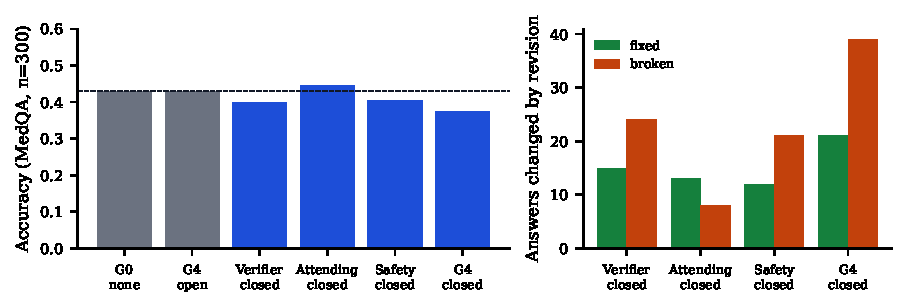
\includegraphics[width=\textwidth]{figures/closed_loop.pdf}
\caption{Left: accuracy per configuration on 300 MedQA questions, with 95\% Wilson intervals (dashed line: G0).
Right: revised answers that changed from wrong to right (fixed) or right to wrong (broken); revisions that kept their
correctness are not shown.}
\label{fig:closed}
\end{figure*}

\subsection{The checks cannot tell right from wrong}
Table~\ref{tab:auroc} treats each check as a detector of a wrong answer. Every AUROC lay between 0.497 and 0.57, close
to chance (0.5); the G4 closed-loop values (0.533 to 0.562) fall in the same range. In every configuration that
included it (G3 closed, G4 open and G4 closed), the safety validator raised at least one alert on all 300 runs, so an
alert carried no information about correctness; even HIGH or CRITICAL alerts alone reached only 0.568.

\begin{table}[t]
\centering
\caption{Each Governance Signal as a Detector of a Wrong Answer}
\label{tab:auroc}
\footnotesize
\begin{tabular}{@{}llrr@{}}
\toprule
\textbf{Signal} & \textbf{Configuration} & \textbf{Fires on} & \textbf{AUROC} \\
\midrule
Ungrounded claim (verifier) & G1 closed & 36.3\% & 0.560 \\
 & G4 open & 35.3\% & 0.497 \\
Any safety alert & G3 closed & 100.0\% & 0.550 \\
 & G4 open & 100.0\% & 0.507 \\
HIGH/CRITICAL safety alert & G3 closed & 31.3\% & 0.568 \\
 & G4 open & 32.7\% & 0.535 \\
Reviewer revise/reject & G2 closed & 34.7\% & 0.570 \\
 & G4 open & 74.7\% & 0.523 \\
\bottomrule
\end{tabular}

\vspace{1mm}
\parbox{\columnwidth}{\footnotesize Fires on: share of the 300 runs in which the signal fired. AUROC 0.5 is chance.
The signal is the first check's alert and the label is whether the final answer is wrong; in closed loop the final
answer may be the revised one.}
\end{table} The
model's own stated confidence was also poorly calibrated (expected calibration error (ECE) 0.2374, Brier score 0.3021). Feeding such signals back
cannot be expected to help: the model is told to reconsider right and wrong answers alike.

\subsection{Cost}
Governance multiplied cost. Mean tokens per question rose from 2200.9 (G0) to 7570.4 (G4 open) and 11362.7 (G4
closed), and median summed latency from 21.2\,s to 142.5\,s. At an illustrative rate of US\$0.10 per million input % numcheck:ignore
and \$0.20 per million output tokens (an assumption fixed in our code, not a quoted provider price), estimated % numcheck:ignore
cost per question rose from \$0.000288 to \$0.001408. Fig.~\ref{fig:tradeoff} shows that no configuration buys
accuracy with this overhead, a cost that could weigh most where compute is limited.

\begin{figure*}[t]
\centering
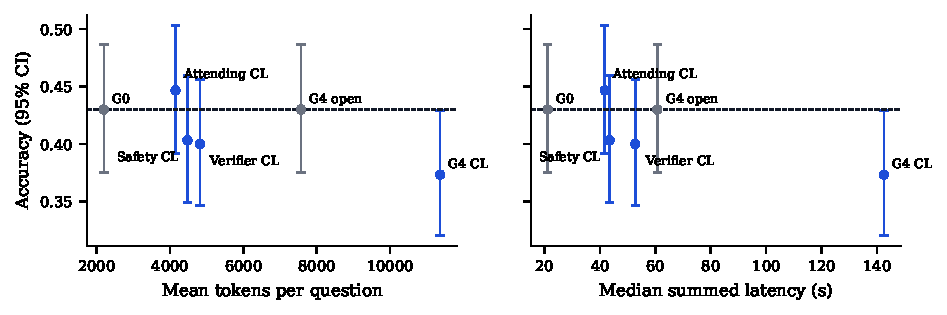
\includegraphics[width=\textwidth]{figures/tradeoff.pdf}
\caption{Accuracy against mean tokens per question (left) and median summed latency (right), with 95\% Wilson
intervals ($n = 300$ each). Dashed line: G0. Grey: open loop; blue: closed loop; marker shapes identify
configurations.}
\label{fig:tradeoff}
\end{figure*}

\subsection{Evaluation shortcuts produced apparent gains}
In our own earlier evaluations, two shortcuts would have changed our conclusions. First, in a 150-case evaluation (Table~\ref{tab:audit}),
substring scoring credited empty and single-letter answers and reported accuracy 0.739; scored correctly it is 0.293.

\begin{table}[t]
\centering
\caption{Earlier 150-Case Evaluation: Reported Versus Audited}
\label{tab:audit}
\footnotesize
\begin{tabular}{@{}lcc@{}}
\toprule
\textbf{Quantity} & \textbf{Reported} & \textbf{Audited} \\
\midrule
Accuracy, all cases & 0.739 & 0.293 \\
Accuracy, 71 cases with a real label & 0.783 & 0.380 \\
Unparsed (empty) diagnoses scored as correct & -- & 216 runs \\
Bare option letters scored 0.9 without options & -- & 395 runs \\
Gold labels that were templated titles & -- & 79 of 150 \\
\bottomrule
\end{tabular}
\end{table} Second, an earlier
\emph{unpaired} closed-loop pass regenerated the first diagnosis for each configuration. The regenerated answer matched
the baseline's in only 79.5\% and 74.6\% of questions, and in that pass the attending reviewer appeared to reach
46.3\% and G4 closed loop 43.0\%. With pairing, these become 44.7\% and 37.3\%. This is one setup and one model, not
a general property of unpaired designs.

% ============================================================
\section{Discussion and Limitations}
% ============================================================
A governance layer is useful only if its alerts are specific enough to act on and acting on them improves the
decision. Here the alerts failed the first test, so closing the loop failed the second: revision moved answers in both
directions and, with every check active, more often in the wrong one. The attending reviewer, the only check whose
revisions fixed more answers than they broke, came closest to helping, though not significantly. Our data suggest that
better-calibrated checks, not more loops, are the bottleneck. This cautions against equating ``more safety agents''
with ``safer'': governance should be validated on paired data before it is relied on.

Limitations: one 11B model from one provider was tested, each question was run once, and no clinician has yet rated
the outputs; the attending reviewer is simulated. With 300 pairs and the mean discordance of our comparisons
(12.9\%), the smallest accuracy difference detectable with 80\% power at \mbox{$\alpha = 0.05$} is 5.8 points, so smaller
effects of single checks cannot be excluded. Cost figures use an assumed token rate. Results may differ for larger
models or checks grounded in drug and guideline databases.

% ============================================================
\section{Conclusion}
% ============================================================
On 300 MedQA questions with a paired design, governance checks did not improve a clinical language model's answers,
and letting all of them trigger revision lowered accuracy from 43.0\% to 37.3\% while multiplying token use. Next we
will repeat the study on a larger model, test better-calibrated checks, and collect blinded clinician ratings.
Code and data: \url{https://github.com/nikshith-nooka/GovMed-AI}. All data are public research questions with no patient
information; the software is not intended for diagnosis or treatment.

% ============================================================
\begin{thebibliography}{00}
\bibitem{singhal2023large}
K.~Singhal et~al., ``Large language models encode clinical knowledge,'' \emph{Nature}, vol.~620, no.~7972, pp. 172--180, 2023, \href{https://doi.org/10.1038/s41586-023-06291-2}{doi: 10.1038/s41586-023-06291-2}.

\bibitem{nori2023capabilities}
H.~Nori, N.~King, S.~M. McKinney, D.~Carignan, and E.~Horvitz, ``Capabilities of GPT-4 on medical challenge problems,'' \emph{arXiv preprint arXiv:2303.13375}, 2023.

\bibitem{rajpurkar2022ai}
P.~Rajpurkar, E.~Chen, O.~Banerjee, and E.~J. Topol, ``AI in health and medicine,'' \emph{Nature Medicine}, vol.~28, no.~1, pp. 31--38, 2022, \href{https://doi.org/10.1038/s41591-021-01614-0}{doi: 10.1038/s41591-021-01614-0}.

\bibitem{hager2024evaluation}
P.~Hager et~al., ``Evaluation and mitigation of the limitations of large language models in clinical decision-making,'' \emph{Nature Medicine}, vol.~30, no.~9, pp. 2613--2622, 2024, \href{https://doi.org/10.1038/s41591-024-03097-1}{doi: 10.1038/s41591-024-03097-1}.

\bibitem{pal2023medhalt}
A.~Pal, L.~K. Umapathi, and M.~Sankarasubbu, ``Med-HALT: Medical domain hallucination test for large language models,'' in \emph{Proc. 27th Conf. Computational Natural Language Learning (CoNLL)}, Singapore, 2023, pp. 314--334, \href{https://doi.org/10.18653/v1/2023.conll-1.21}{doi: 10.18653/v1/2023.conll-1.21}.

\bibitem{hong2023metagpt}
S.~Hong et~al., ``MetaGPT: Meta programming for a multi-agent collaborative framework,'' in \emph{Proc. ICLR}, Vienna, Austria, 2024.

\bibitem{wu2023autogen}
Q.~Wu et~al., ``AutoGen: Enabling next-gen LLM applications via multi-agent conversations,'' in \emph{Proc. Conf. Language Modeling (COLM)}, 2024.

\bibitem{chen2023agentverse}
W.~Chen et~al., ``AgentVerse: Facilitating multi-agent collaboration and exploring emergent behaviors,'' in \emph{Proc. ICLR}, Vienna, Austria, 2024.

\bibitem{du2023improving}
Y.~Du, S.~Li, A.~Torralba, J.~B. Tenenbaum, and I.~Mordatch, ``Improving factuality and reasoning in language models through multiagent debate,'' in \emph{Proc. ICML}, PMLR vol.~235, 2024, pp. 11733--11763.

\bibitem{bedi2025optimization}
S.~Bedi, I.~Mlauzi, D.~Shin, S.~Koyejo, and N.~H. Shah, ``The optimization paradox in clinical AI multi-agent systems,'' \emph{arXiv preprint arXiv:2506.06574}, 2025.

\bibitem{jin2021medqa}
D.~Jin, E.~Pan, N.~Oufattole, W.-H. Weng, H.~Fang, and P.~Szolovits, ``What disease does this patient have? A large-scale open domain question answering dataset from medical exams,'' \emph{Applied Sciences}, vol.~11, no.~14, Art. no. 6421, 2021, \href{https://doi.org/10.3390/app11146421}{doi: 10.3390/app11146421}.

\bibitem{jin2019pubmedqa}
Q.~Jin, B.~Dhingra, Z.~Liu, W.~W. Cohen, and X.~Lu, ``PubMedQA: A dataset for biomedical research question answering,'' in \emph{Proc. EMNLP-IJCNLP}, Hong Kong, China, 2019, pp. 2567--2577, \href{https://doi.org/10.18653/v1/D19-1259}{doi: 10.18653/v1/D19-1259}.

\bibitem{tang2024medagents}
X.~Tang et~al., ``MedAgents: Large language models as collaborators for zero-shot medical reasoning,'' in \emph{Findings of ACL}, Bangkok, Thailand, 2024, pp. 599--621, \href{https://doi.org/10.18653/v1/2024.findings-acl.33}{doi: 10.18653/v1/2024.findings-acl.33}.

\bibitem{kim2024mdagents}
Y.~Kim et~al., ``MDAgents: An adaptive collaboration of LLMs for medical decision-making,'' in \emph{Advances in Neural Information Processing Systems}, vol.~37, 2024, pp. 79410--79452.

\bibitem{zhu2025medagentboard}
Y.~Zhu et~al., ``MedAgentBoard: Benchmarking multi-agent collaboration with conventional methods for diverse medical tasks,'' in \emph{Proc. NeurIPS Datasets and Benchmarks Track}, 2025.

\bibitem{rebedea2023nemo}
T.~Rebedea, R.~Dinu, M.~N. Sreedhar, C.~Parisien, and J.~Cohen, ``NeMo Guardrails: A toolkit for controllable and safe LLM applications with programmable rails,'' in \emph{Proc. EMNLP: System Demonstrations}, Singapore, 2023, pp. 431--445, \href{https://doi.org/10.18653/v1/2023.emnlp-demo.40}{doi: 10.18653/v1/2023.emnlp-demo.40}.

\bibitem{zheng2023judging}
L.~Zheng et~al., ``Judging LLM-as-a-judge with MT-Bench and Chatbot Arena,'' in \emph{Advances in Neural Information Processing Systems (Datasets and Benchmarks Track)}, vol.~36, 2023, pp. 46595--46623.

\bibitem{mcnemar1947note}
Q.~McNemar, ``Note on the sampling error of the difference between correlated proportions or percentages,'' \emph{Psychometrika}, vol.~12, no.~2, pp. 153--157, 1947, \href{https://doi.org/10.1007/BF02295996}{doi: 10.1007/BF02295996}.

\bibitem{efron1979bootstrap}
B.~Efron, ``Bootstrap methods: Another look at the jackknife,'' \emph{The Annals of Statistics}, vol.~7, no.~1, pp. 1--26, 1979, \href{https://doi.org/10.1214/aos/1176344552}{doi: 10.1214/aos/1176344552}.

\bibitem{holm1979simple}
S.~Holm, ``A simple sequentially rejective multiple test procedure,'' \emph{Scandinavian Journal of Statistics}, vol.~6, no.~2, pp. 65--70, 1979.
\end{thebibliography}

\end{document}
